\chapter{Tri par fusion}
\section{Description de l’objectif de l’algorithme}
En informatique, un tableau est une structure de données représentant une séquence finie d’éléments définis par un index représentant leurs positions au sein du tableau. 
C’est un type de conteneur que l’on retrouve dans un grand nombre de langages de programmation et est l’un des plus utilisés dû à sa simplicité. Les données du tableau étant accessible individuellement il est nécessaire de faire une recherche lorsque l’on souhaite accéder a une valeur spécifique du tableau. Cependant, lorsque la taille de la structure est grande il devient difficile d’y accéder efficacement.
\section{Fonctionnement de l'algorithme}
Le tri par fusion aussi appeler tri dichotomique est un exemple classique d’algorithme de division pour régner. 
L’opération principale de l’algorithme est la fusion, qui consiste à réunir deux listes triées en une seule. L’efficacité de l’algorithme vient du fait que deux listes triées peuvent être fusionnées en temps linéaire . On peut résumer son fonctionnement en deux étapes :
\par
\begin{enumerate}
  \item Divisez la liste non triée en sous-listes jusqu'à ce qu'il y ait N sous-listes avec un élément dans chacune (N est le nombre d'éléments dans la liste non triée).
  \item Fusionnez les sous-listes deux à la fois pour produire une sous-liste triée, répétez cette opération jusqu'à ce que tous les éléments soient inclus dans une seule liste.
\end{enumerate}

\begin{figure}[H]
    \centering
        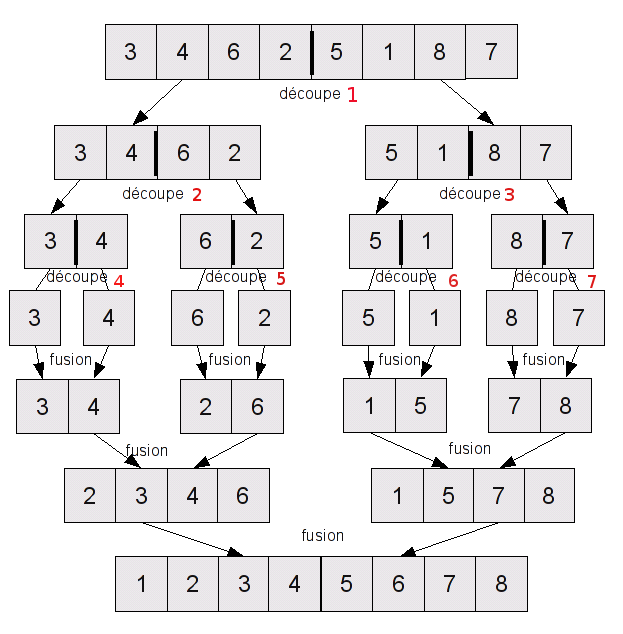
\includegraphics[scale=0.7]{ressources/fusion.png}
        \caption{Exemple graphique d’un tri par fusion}
    \label{fig:fusion}
\end{figure}
\par
Afin d’optimiser le déroulement du tri, nous utilisons 2 fonctions distinctes. Une fonction TriFusion qui divise le tableau récursivement et une fonction Fusion qui elle trie les sous tableaux
avant de les fusionner à nouveau. Nous pouvons le représenter via le pseudo code suivant :
\par
\begin{function}[H]
    \textbf{Variables :}\\
    TabG, TabD : tableau d'entier\;
    SousTab1, SousTab2, SousTab1Index, SousTab2Index, SousTabFusionIndex : entier\;
    \Begin{
        $milieu \leftarrow \frac{droite + gauche}{2}$\;
        $SousTab1  \leftarrow milieu - gauche + 1$\;
        $SousTab2  \leftarrow droite - milieu$\;
        \For{$i \leftarrow 1$ \KwTo $SousTab1$}{
            $tabG[i] \leftarrow tab[gauche + i]$\;
        }
        \For{$j \leftarrow 1$ \KwTo $SousTab2$}{
            $tabG[j] \leftarrow tab[mid + 1 + j]$\;
        }
        $SousTab1  \leftarrow 0$\;
        $SousTab2  \leftarrow 0$\;
        $SousTabFusionIndex  \leftarrow gauche$\;
        \While{$SousTab1Index < SousTab1$ et $SousTab2Index < SousTab2$}
       {
            %\\
            \uIf{tabG[SousTab1Index] <= tabD[SousTab2Index]}{
                $tab[SousTabFusionIndex] \leftarrow tabG[SousTab2Index]$\;
                $SousTab1Index++$\;
            }
            \Else {
                $tab[SousTabFusionIndex] \leftarrow tabD[SousTab2Index]$\;
                $SousTab2Index++$\;
            }
            $SousTabFusionIndex++$\;
        %\EndWhile
        }
        \While{$SousTab1Index < SousTab1$}
       {
            %\\
            $tab[SousTabFusionIndex] \leftarrow tabG[SousTab1Index]$\;
            $SousTab1Index++$\;
            $SousTabFusionIndex++$\;
        %\EndWhile
        }
        \While{$SousTab2Index < SousTab2$}
       {
            %\\
            $tab[SousTabFusionIndex] \leftarrow tabG[SousTab2Index]$\;
            $SousTab1Index++$\;
            $SousTabFusionIndex++$\;
        %\EndWhile
        }
    }
    \caption{Fusion(Entrée: tab: tableau d'entier; droite, gauche: entier;)}
\end{function}

\begin{function}[H]
    \textbf{Variables :}\\
    milieu : entier\;
    \Begin{
        \tcp{On divise le tableau en 2 de manière recursive puis on les tri avant de les fusionner}
        \If{$debut >= fin$}
            {retour\;}
        \tcp{On calcule l'index du milieu du tableau}
        $milieu \leftarrow debut + (fin - debut) / 2$\;
        TriFusion(tab, debut, milieu)\;
        TriFusion(tab, milieu + 1, fin)\;
        \tcp{On utilise la fonction fusion pour trier puis fusioner les sous tableaux en un seul tableau trié}
        Fusion(tab, debut, mid, fin)\;
    }
    \caption{TriFusion(Entrée: tab: tableau d'entier; debut, fin: entier;)}
\end{function}

\section{Calcul de complexité}

\subsection{Complexité temporelle}
la fonction merge consiste a decouper une liste de taille N en N sous-listes avec un élément dans chacune donc on doit parcourir tout le tableau qui est donc de complexite O(n). 
\subsubsection{Complexité d'une fonction récursive}
Pour calculer la complexité d'une fonction récursive, il faut souvent utiliser une formule de récurrence. 
apres la division , on aura deux problemes a résoudre de taille N/2.
On les résout récursivement 
on exprime donc la complexité au pire cas de merge sort par n(log n + 1) 
quelque soit l'order des elements de tableau , le tri fusion consiste toujour a le decouper en sous listes jusqu'a ce qu'il ya que des feuilles et les fusionner .
\textbf{et donc La complexité de tri par fusion est toujours( meilleur , moyenne et pire cas) égale à : O(nln(n)).}
\\
\par
le tableau suivant représente les temps d’exécution théorique en nanoseconde de l’algorithme selon la variation de la taille de l’expression :
\small
\begin{center}
\begin{tabular}{| c | c | c | c | c | c | c | c | c | c | c | c | c |}
    \hline
    N &  10 & 50 & 100 & 500 & 1000 & 5000 & 10000 & 100000 & 1000000 & 10000000 \\
    \hline
    t(ns) & 10 &
84.95&
200&
1349.48&
3000&
18494.85&
40000&
500000&
6000000&
70000000 \\
    \hline
\end{tabular}  
\end{center}
\par
La figure suivante représente l’évolution du temps d’exécution selon la longueur du tableau: 
\begin{figure}[H]
    \centering
        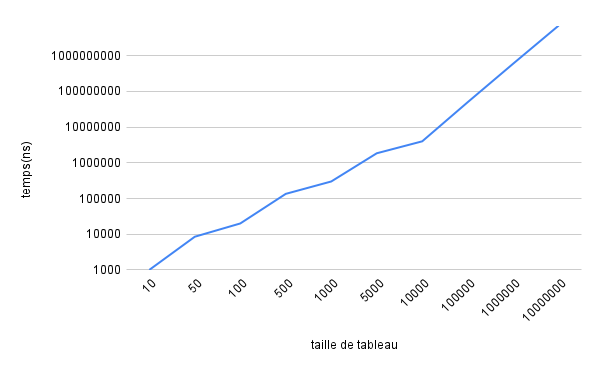
\includegraphics[scale=0.7]{ressources/chartfusiontheorique.png}
        \caption{Temps d'exécution théorique du programme selon la longueur du tableau}
    \label{fig:temps_exec_dico_theo}
\end{figure} 
\subsection{Complexité spatiale}
la complexite spatiale de tri fusion est O(n).
\section{Experimentation}
Le tableau suivant représente les temps d’exécution en nanoseconde de l’algorithme selon la variation de la taille et la configuration de l'entree .
\subsubsection{Les données du tableau sont triées en ordre inverse.}
\small
\begin{center}
\resizebox{19cm}{!}{
\begin{tabular}{| c | c | c | c | c | c | c | c | c | c | c |}
    \hline
    N &  10000 & 50000 & 100000 & 500000 & 1000000 & 5000000 & 10000000 & 50000000 \\
    \hline
    t1(s) & 0.00042 &	0.002448 &	0.00494 &	0.025386 &	0.055339&	0.304839 & 0.603316&	3.768904 \\
    \hline
    t2(s) & 0.000808 &	0.004676 &	0.009942&	0.052479&	0.113005&	0.624881 & 1.28433&	7.613348  \\
    \hline
    t3(s) & 0.001207 &	0.00691	&0.014647&	0.081096&	0.169904&	0.944664 & 1.942545	&11.444372  \\
    \hline
    t4(s) & 0.001619&	0.009289&	0.019483&	0.10869&	0.227738&	1.259653 & 2.613055&	15.351673  \\
    \hline
    t5(s) & 0.001993&	0.011645&	0.024382&	0.133484&	0.284621&	1.568324 & 3.303382	&19.305843  \\
    \hline
    t6(s) & 0.00238	&0.013891&	0.029357&	0.160016&	0.342119&	1.905382 & 3.922201&	23.20739  \\
    \hline
    t7(s) & 0.002792&	0.016027&	0.034042&	0.186831&	0.400959&	2.220602 & 4.579432&	27.165472  \\
    \hline
    t8(s) & 0.003176&	0.017979&	0.038603&	0.213543&	0.459195&	2.531605 & 5.232867	&31.079348 \\
    \hline
    t9(s) & 0.003569&	0.020067&	0.043068&	0.241344&	0.512189&	2.844363 & 5.811679&	34.919087 \\
    \hline
    t10(s) & 0.003952&	0.022506&	0.047414&	0.268108&	0.569763&	3.172519 & 6.390016	&38.880528  \\
    \hline
    Moyenne(s) & 0.002192&	0.012544&	0.026588&	0.147098&	0.313483&	1.737683 & 3.568282	&21.273597  \\
    \hline
\end{tabular}}
\end{center}
\normalsize
\subsubsection{Les données du tableau sont triées en bon ordre.}
\small
\begin{center}
\resizebox{19cm}{!}{
\begin{tabular}{| c | c | c | c | c | c | c | c | c | c | c |}
    \hline
    N &  10000 & 50000 & 100000 & 500000 & 1000000 & 5000000 & 10000000 & 50000000 \\
    \hline
    t1(s) & 0.000569&	0.002628&	0.005863&	0.030151&	0.061241&	0.360749&	0.709762	&4.124928 \\
    \hline
    t2(s) & 0.001068&	0.005192&	0.011261&	0.059449&	0.121092&	0.682264&	1.400675&	8.280286  \\
    \hline
    t3(s) & 0.001561&	0.007656&	0.016423&	0.088011&	0.176175&	1.001632&	2.058852&	12.254911  \\
    \hline
    t4(s) & 0.00202	&0.010261&	0.021879&	0.11565&	0.228058&	1.310229&	2.746449&	15.998439  \\
    \hline
    t5(s) & 0.002476&	0.012919&	0.027025&	0.144914&	0.283809&	1.661196&	3.447879&	19.919397  \\
    \hline
    t6(s) & 0.002887&	0.015353&	0.032353&	0.1737&	0.341154&	2.013703&	4.154876&	23.882657  \\
    \hline
    t7(s) & 0.003342&	0.017781&	0.037866&	0.202648&	0.398567&	2.376409&	4.836434&	27.617182  \\
    \hline
    t8(s) & 0.003832&	0.02029&	0.043166&	0.232642&	0.459596&	2.74455&	5.524018&	31.593124 \\
    \hline
    t9(s) & 0.004247&	0.022741&	0.048409&	0.262612&	0.511865&	3.105877&	6.199981&	35.648717 \\
    \hline
    t10(s) & 0.004753&	0.025202&	0.053627&	0.292089&	0.564445&	3.421129&	6.906015&	39.616554  \\
    \hline
    Moyenne(s) & 0.002675&	0.014002&	0.029787&	0.160187&	0.3146&	1.867774&	3.798494&	21.89362  \\
    \hline
\end{tabular}}
\end{center}
\normalsize
\par
\subsubsection{Les données du tableau sont aleatoires.}
\small
\begin{center}
\resizebox{19cm}{!}{
\begin{tabular}{| c | c | c | c | c | c | c | c | c | c | c |}
    \hline
    N &  10000 & 50000 & 100000 & 500000 & 1000000 & 5000000 & 10000000 & 50000000 \\
    \hline
    t1(s) & 0.000659&	0.003734&	0.007724&	0.044176&	0.082721&	0.449917&	1.040069&	5.768796 \\
    \hline
    t2(s) & 0.001049&	0.006208&	0.012345&	0.074345&	0.140179&	0.734552&	1.777799&	9.790986  \\
    \hline
    t3(s) & 0.001447&	0.00852&	0.01707&	0.103247&	0.197034&	1.049007&	2.509943&	13.84349  \\
    \hline
    t4(s) & 0.001784&	0.011054&	0.02166&	0.132922&	0.252066&	1.37088&	3.239306&	17.834287  \\
    \hline
    t5(s) & 0.002294&	0.013381&	0.026351&	0.16232&	0.307356&	1.704408&	3.973541&	21.750978  \\
    \hline
    t6(s) & 0.002644&	0.015765&	0.030871&	0.192797&	0.365797&	2.039695&	4.707078&	25.682164  \\
    \hline
    t7(s) & 0.00303&	0.018165&	0.035004&	0.222074&	0.420898&	2.385981&	5.453311&	29.653989 \\
    \hline
    t8(s) & 0.003439&	0.020634&	0.039404&	0.249832&	0.480518&	2.729575&	6.194547&	33.541621 \\
    \hline
    t9(s) & 0.003828&	0.022892&	0.043711&	0.278123&	0.542099&	3.078519&	6.927452&	37.484699 \\
    \hline
    t10(s) & 0.004228&	0.02522&	0.048058&	0.307679&	0.596437&	3.417302&	7.677789&	41.405992  \\
    \hline
    Moyenne(s) & 0.00244&	0.014557&	0.02822&	0.176752&	0.338511&	1.895984&	4.350083&	23.6757  \\
    \hline
\end{tabular}}
\end{center}
\normalsize
\par
La figure suivante représente l’évolution du temps d’exécution en (s) selon la taille et la configuration du tableau :
\begin{figure}[H]
    \centering
        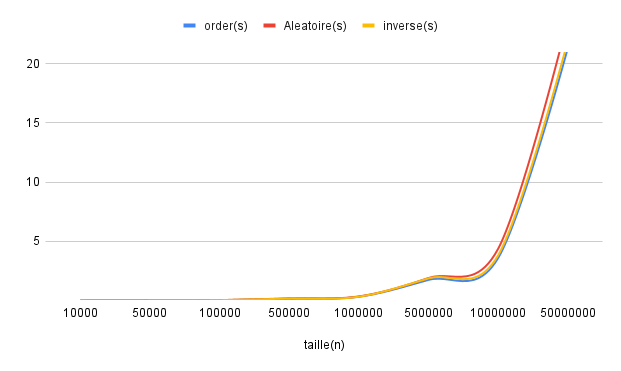
\includegraphics[scale=0.7]{ressources/chartfusion.png}
        \caption{Temps d'exécution du programme selon la taille du tableau}
    \label{fig:temps_exec_dico_theo}
\end{figure} 
\par
Depuis les graphes, on observe que le temps d’exécution évolue de manière linéairethemtique avec l’augmentation de la taille du tableau quelque soit l'ordre, ce qui correspond bien à la complexité théorique calculée auparavant.

\par
\section{Conclusion}
D'apres l'etude theorique et experimentale de la fonction tri fusion on observe que le temps d'execution evolue de maniere lineairethemtique avec l'augmentation de la taille du tableau quelque soit la configuration utilisee , O(nlog(n)) est pratiquement une complexite optimale pour les configuration inverse et aleatoire mais il y'a meilleur fonctions de tri avec une complexite plus optimale lorsque on parle de la configuration en bon ordre.
